 \documentclass[12pt]{article}

\usepackage{fancyhdr}
\usepackage{geometry}
\usepackage[utf8]{inputenc}
\usepackage[T1]{fontenc}
\usepackage[english]{babel}
\usepackage{amsmath,amssymb,amstext}
\usepackage{hyperref}
\usepackage{cancel}
\usepackage{dsfont}
\usepackage{physics}
\usepackage{mathrsfs}
\usepackage{lmodern}
\usepackage{enumerate}
\usepackage{enumitem}
\usepackage{graphicx}
\usepackage{listings, color}
\usepackage[labelfont=bf]{caption}
\usepackage{titling}
\usepackage{siunitx}
\usepackage{tikz}
\usepackage{icomma}
\usepackage{revsymb}
\usepackage{overpic}
\usepackage{subcaption}

\usepackage[backend=biber,backref=false,style=numeric-comp, sorting=none,block=ragged,firstinits=true]{biblatex}


\lstset{basicstyle=\scriptsize,breaklines=true}



%Geometrie----------------------------------------------------------------------------------------------------------

\geometry{a4paper, top=25mm, left=15mm, right=15mm, bottom=25mm,headsep=10mm, footskip=10mm}
\pagestyle{fancy}
\setlength{\parindent}{0pt} %Zeileneinrückung

\fancyhf{} %Setzt voreingestellte Kopf-und Fußzeilen-Eigenschaften zurück

\lhead{\nouppercase{\leftmark}}
\chead{}
\rhead{\thepage}

\lfoot{}
\cfoot{}
\rfoot{}

\title{\vspace{0cm}{\Huge Applied Physics Master Lab:\\ \vspace{1cm} Diamonds for Sensing Applications}}
\author{Cristian Medina\\Simon Stephan}
\date{conducted from 28.05.2018 to 01.06.2018}

\pretitle{%
	\begin{center}
		\LARGE
		
\includegraphics[width=6cm,]{../figures/siegel}\\[\bigskipamount]
	}
	\posttitle{\end{center}}

%neue Commands----------------------------------------------------------------------------------------------------------
\newcommand{\nab}{\vec{\nabla}} %direkter Befehl mit Vektorpfeil
\newcommand{\sinc}{\mathrm{sinc}}
\newcommand{\degree}{^\circ}

\newcommand{\del}[2][]{\frac{\partial #1}{\partial #2}}
\newcommand{\code}[1]{\texttt{#1}}

\addbibresource{fp_refs.bib}

%Titel,Inhalt----------------------------------------------------------------------------------------------------------

\begin{document}
	

	
	\pagenumbering{gobble} %verstecke Seitenzahl
	\maketitle
	\newpage
	
	
	
	\section*{Abstract}

Hello Cris

hello simon

	
	\newpage
	
	\thispagestyle{empty}
	\tableofcontents
	\newpage
	
	%Schreiben----------------------------------------------------------------------------------------------------------
	\pagenumbering{arabic}
	
	% !TeX spellcheck = en_GB
\section{Introduction}

Diamonds are not just known and appreciated by their beauty but also for it important technical properties like their mechanical hardness which they mainly get from their crystal structure. Nevertheless there are defects in their lattice structure which enable us to use diamonds more variously. Colour centres, for example, are fluorescent lattice defects which can be used for many sensing applications \cite{anleitung}. In this experiment we will examine the properties of the so-called nitrogen vacancy (NV) centre and it's sensitivity to magnetic fields.\\

Colour centres (CC) are  regular spacing in the lattice that absorbs a particular colour in light. Each CC involves the absence of an atom from the place it would normally occupy in the solid and the relation of an electron with such an empty place, or vacancy. Solids without colour centres may still have colour if impurity atoms or other structures that absorb light are present.

 getting lifted into an excited state and then decaying back into the ground state by emitting a photon with a wavelength in the visible range which gives the diamond their many different colours. The fluorescence of the here examined NV-centres can be used to detect magnetic fields.\\

This is done using the measurement method of optically detected magnetic resonances (ODMR) in which the NV-centre is excited by microwaves which leads to a loss in fluorescence at a certain microwave frequency. The recorded frequency spectrum in a frequency range around that frequency depends on the external magnetic field.\\

Also the fluorescence spectrum of the diamond as well as its size will be measured using an optical spectrometer and a CCD camera.
	\newpage
	\section{Theoretical Background}
In the following some physical concepts needed for the understanding of this experiment are explained.
%\subsection{Physical Concepts}
\subsection{Colour Centres}


\subsection{NV-Centres in Diamonds}

%\subsection{Experimental Methods}
\subsection{Optically Detected Magnetic Resonance}
	\newpage
	\section{Experimental Set-up and Procedure}
\subsection{Set-Up}

\subsection{Calibration}
\subsubsection{convertion factor camera}
The strip was meassure with a calibrator at $1.2\pm 0.1\,\mathrm{mm}$ and the camara used was a Thorlabs CCD camera with dimentions of 1280x1024 pixels, each pixel with $5.2\times5.2 \mathrm{\mu m}$ according to the manufacturer.
In order to know the actual resolution of our microscope a calibration was done based on the magnification and calibration factor of the set up.
Theoritically our $C_{f}$ can be calculated as:
\\

\begin{equation}
C_{f}=\dfrac{1 px \cdot M}{d_{p}} = 1552 px/mm
\end{equation}\\
Where $M$ is the magnification and $d_{p}$ is the pixel sizes. And with a Magnification icual to the lenses used for the confocal setup is equal to the magnification $M=f2/f1=8$.
In this case the tool of Thorlab’s software was used to determine and measure the width of the microstrip. Using the equation above and the respective measumente we denote that  $C_{f} =1346 \,\mathrm{px/mm}$, with a magnification factor close to $M=7X$.


\subsubsection{Electronic components}

In order Performe our ODMR, is crucial to determine the amount of microwave power deployed into the microstrip and the diamonds. we can not have an absolut power that is been pluging into the set up. The microstrip by defoult have some transmition $T_{Ms}$ and reflecctions $R_{Ms}$ that are unkown.
For this a power coupler was added to the setup and four meassument with diferents arranges where performed as shown in the fig...
First, the power coupler was conected to the DSA in out- out possition to knoe the transmitio of it, $T_{cpl}$. on the other hand the secon setup is an Out conection to the DSA and help to determine the reflection of the CPL $R_{cpl}$. for the thirt and fouth display, the mmicrostrip was added, in the Out-Out possition ( CPL-DSA), messurion the Reflection $R_{cpl-Ms}$ and transmition $T_{cpl-Ms}$ of the hole set.

\begin{figure}
	\centering
	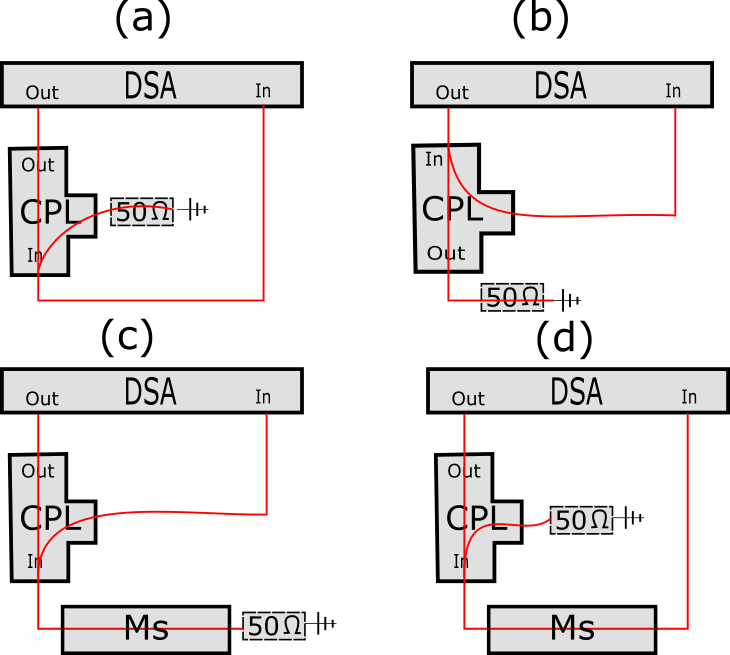
\includegraphics[width=0.7\linewidth]{../figures/APD}
	\caption[diferent arranges of the CPL and MicroStrip conected to the DSA]{(A) CPL conected to the DSA in Out-Out direction messuring $T_{cpl}$, (b) Cpl conected in Out-In secuence and meassuring $R_{cpl}$, (c) CPl and microstrip conected in Out-Out mode and measuring the $R_{cpl-Ms}$ (d) CPL and Microstrip conected in Out-Out moded and meassuring $T_{cpl-Ms}$}
	\label{fig:apd}
\end{figure}

The DSA was set at 0 Dbm and a sweep centered at 2.8GHz frequancy. A 50$\Omega$ resistance was used for the losses ends as shown. The next figure display the four signals of the diferent arranges.
\begin{figure}
	\centering
	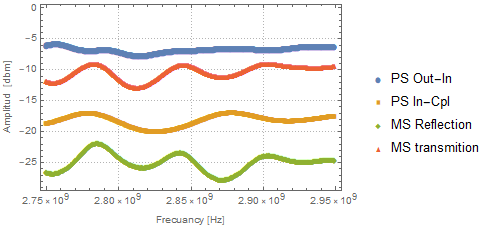
\includegraphics[width=0.7\linewidth]{../figures/microstrip}
	\caption{Atenuattion od the power at 0dBm from top to bottom: $T_{CPL}$,$T_{Cpl-Ms}$, $R_{CPL}$ and $R_{Cpl-MS}$}
	\label{fig:microstrip}
	\end{figure}

The total transmition and reflection ws simply calculated by a sustraction of the Ms trasmition in the diferent processes as next.
\begin{equation}
T_{Ms}=T_{cpl-Ms}-T_{cpl}\\
R_{MS}=R_{cpl-Ms}+T_{cpl}-R_{cpl}
\end{equation}

The atenuation in this cases for the transmiition remains close to cero, specially in the center of the sweep while the reflection as shown reducs drastricly. This gives  us the facts that the power trasmited is close to the 0dBm used in the DSA and few of it is been reflected.

\begin{figure}
	\centering
	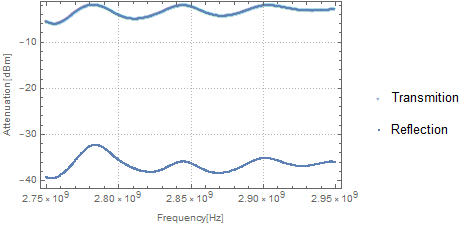
\includegraphics[width=0.7\linewidth]{../figures/microstrip-trasm-eflect}
	\caption[trans-refl]{Ateniation of the resultant transmition (top) and reflectrion (bottom) at the Micristrip, at 0dBm in a 2.8GHZ frequency center.}
	\label{fig:microstrip-trasm-eflect}
\end{figure}







\subsection{Measurements}
	\newpage
	% !TeX spellcheck = en_GB
\section{Evaluation}
\subsection{Calibration}
\subsubsection{Laser Power}

\begin{figure}
	\centering
	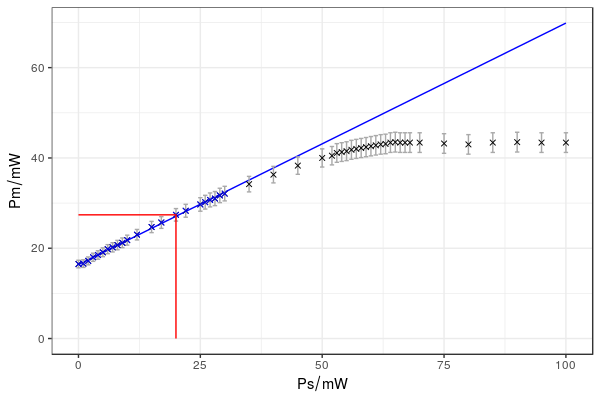
\includegraphics[width=\textwidth]{../figures/powercal.png}
	\caption{Measurement of the laser power}
	\label{fig:power}
\end{figure}

\subsubsection{Optical Spectrometer}
\begin{figure}
	\centering
	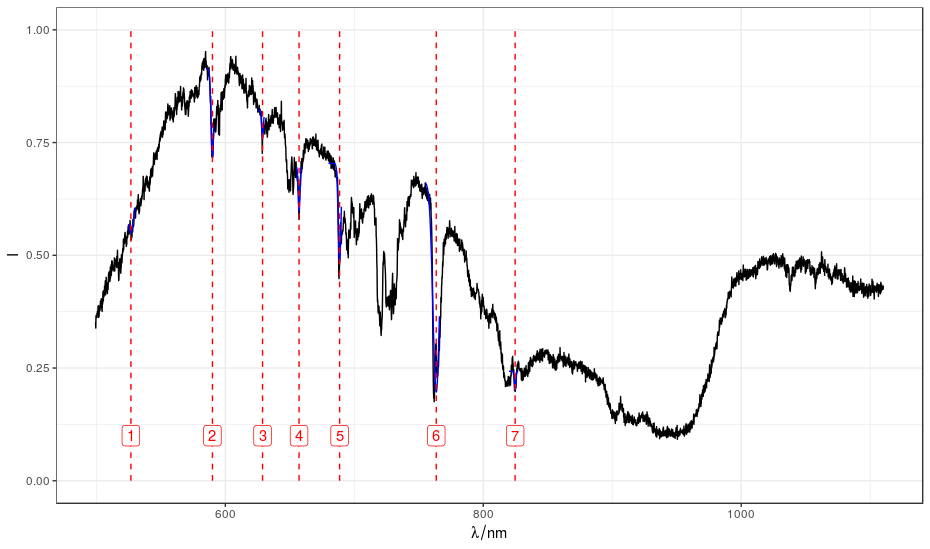
\includegraphics[width=\textwidth]{../figures/sunspectrum.png}
	\caption[Spectrum of the sun with identified Fraunhofer lines]{Spectrum of the sun with identified Fraunhofer lines for calibration of the optical spectrometer}
	\label{fig:sunspectrum}
\end{figure}

\begin{table}
	\centering
	\begin{tabular}{c|c|c|c|c}
		Peak&Position&Element&Position \cite{fraunhoferlines}&Difference\\
		1&$526.8\pm1.7$&Fe I&527.0&$-0.2$\\
		2&$590.0\pm0.5$&Na I&589.6&$+0.4$\\
		3&$628.9\pm0.3$&Fe I&630.3&$-1.4$\\
		4&$657.2\pm0.3$&H $\alpha$&656.3&$+0.9$\\
		5&$688.6\pm0.5$&&&\\
		6&$763.5\pm1.3$&&&\\
		7&$824.7\pm0.3$&&&\\
	\end{tabular}
	\caption{Positions of the Fraunhofer Lines compared to the literature values}
	\label{tab:fraunhofer}
\end{table}

\begin{figure}
	\centering
	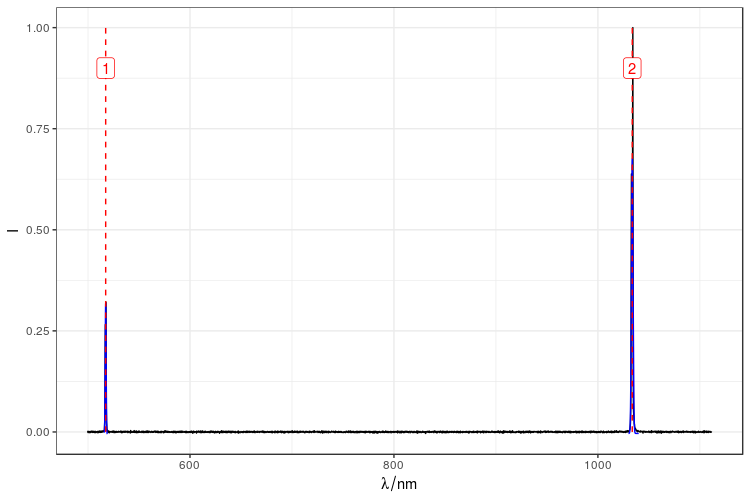
\includegraphics[width=\textwidth]{../figures/laserspectrum.png}
	\caption[Spectrum of the laser]{Spectrum of the laser with identified peaks at the wavelengths $\lambda=(517.3\pm0.2)\,\mathrm{nm}$ and $\lambda=(1033.7\pm0.4)\,\mathrm{nm}$}
	\label{fig:laserspectrum}
\end{figure}

\subsubsection{ODMR calibrations}
\paragraph{Shielding}
\begin{figure}
	\begin{subfigure}{0.5\textwidth}
		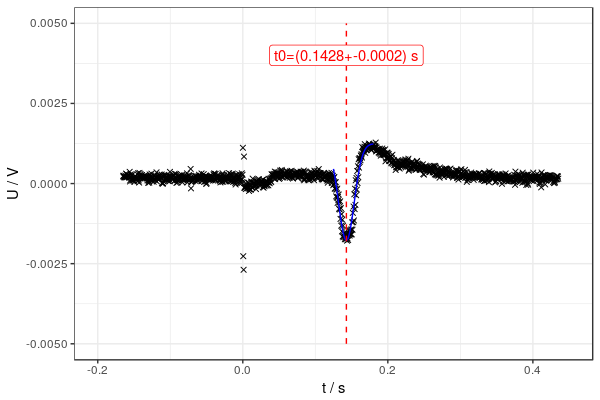
\includegraphics[width=\textwidth]{../figures/odmr-cal-1.png}
		\subcaption{without shielding}
	\end{subfigure}
		\begin{subfigure}{0.5\textwidth}	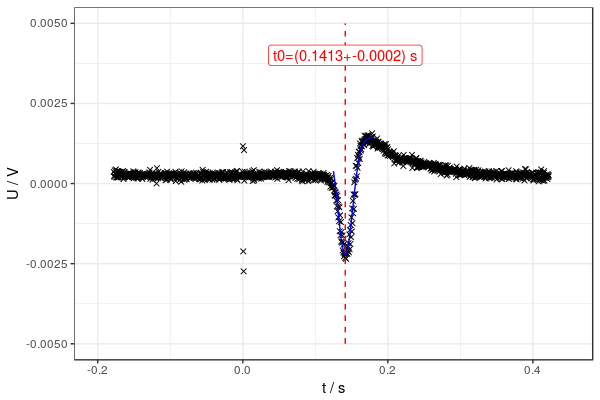
\includegraphics[width=\textwidth]{../figures/odmr-cal-2.png}
		\subcaption{with shielding}
	\end{subfigure}
	\caption{ODMR spectrum}
	\label{fig:odmr-shield}
\end{figure}
\paragraph{Time-to-Frequency Conversion}

\begin{figure}
	\begin{subfigure}{0.5\textwidth}
		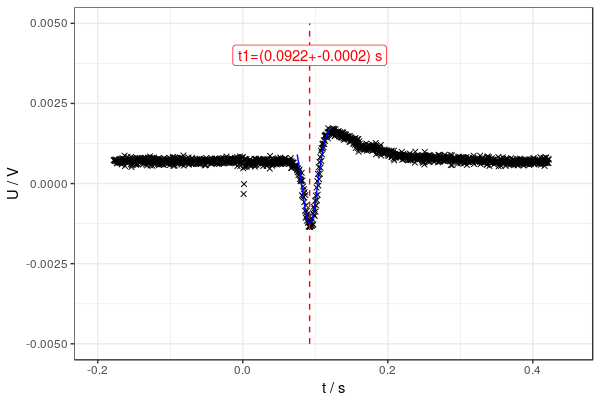
\includegraphics[width=\textwidth]{../figures/odmr-cal-4.png}
		\subcaption{shifted to the left}
	\end{subfigure}
	\begin{subfigure}{0.5\textwidth}
		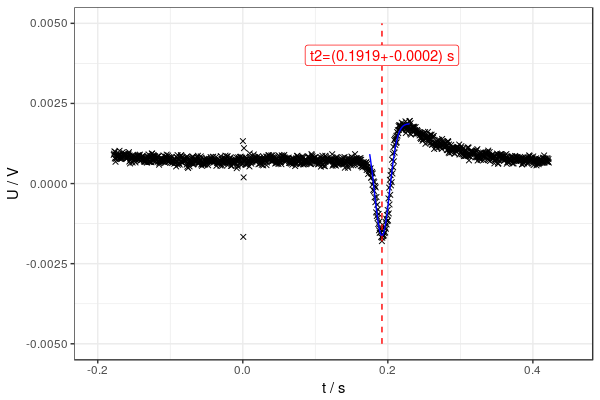
\includegraphics[width=\textwidth]{../figures/odmr-cal-3.png}
		\subcaption{shifted to the right}
	\end{subfigure}
	\caption{ODMR spectrum for time-to-frequency calibration}
	\label{fig:odmr-shift}
\end{figure}

Performing ODMR measurements we achieve the ODMR spectra on the oscilloscope. Therefore the spectra are time-resolved. To gain frequency-resolved spectra we need to calculate the conversion factor from time to frequency. We do this by performing two sweeps with shifted centre frequencies which allows us to calculate the conversion factor and also the offset since we know the frequency at which the peak appears.

The conversion can be expressed by the following equation:

\begin{align}
	f(t)&=\frac{f(t_1)(t_1-t_2)-(f(t_1)-f(t_2))t_1}{t_1-t_2}+\frac{f(t_1)-f(t_2)}{t_1-t_2}\cdot t
\end{align}

Inserting the values achieved from figure \ref{fig:odmr-shift} we get the following conversion function:

\begin{align}
	f(t)&=(1.003\pm0.003)\,\mathrm{\frac{GHz}{s}}\cdot t+(2.708\pm0.011)\,\mathrm{GHz}
\end{align}

Later in this document all spectra are converted by this function and therefore shown in the frequency domain. The errors are gained from the fit and propagated using Gaussian error propagation.

\subsection{Size of the Diamonds}

\subsection{Fluorescence Spectrum}
\begin{figure}
	\centering
	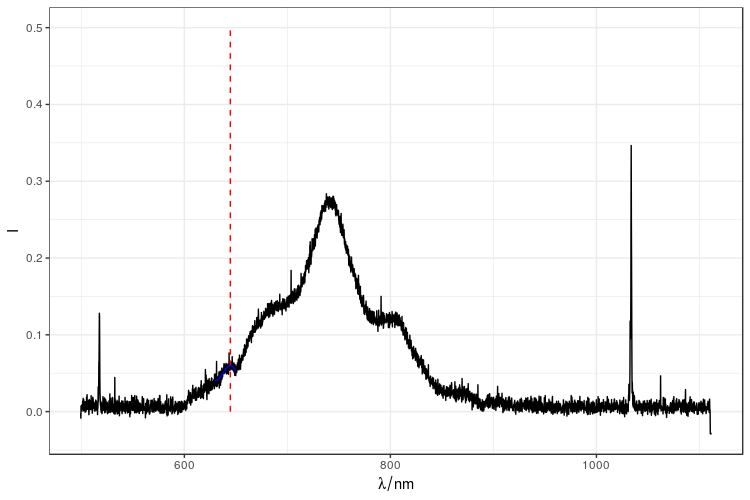
\includegraphics[width=\textwidth]{../figures/fluorescence.png}
	\caption[Fluorescence spectrum of the diamond]{Fluorescence spectrum of the diamond with the zero phonon line (red line) at $\lambda=(645\pm3)\,\mathrm{nm}$. The spectrum was achieved by averaging over 10 measurements.}
	\label{fig:fluorescence}
\end{figure}

\subsection{ODMR Measurements}
\begin{figure}
	\centering
	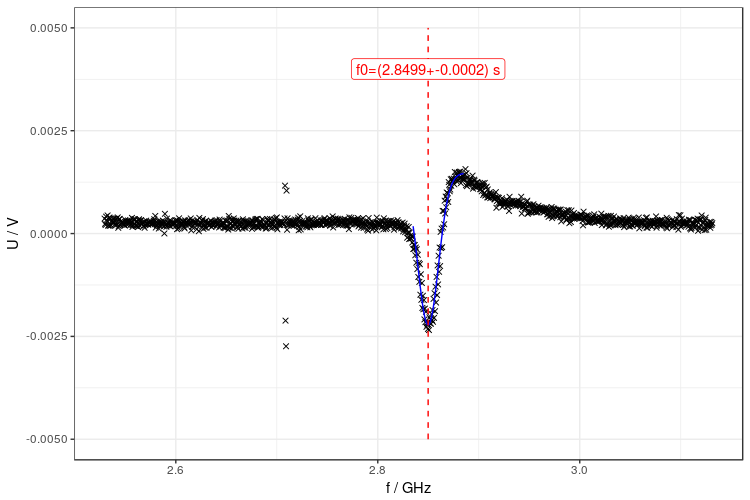
\includegraphics[width=0.8\textwidth]{../figures/odmr-1.png}
	\caption{ODMR Measurement of the diamond without B-Field}
	\label{fig:odmr-no-B}
\end{figure}
	\newpage
	\section{Summary and Discussion}
\label{sec:summary}

%%%%IMPORTANT: Explain reasons for shifted center resonance frequency with B-field
	\newpage
	\section{Appendix}
\subsection{Lab Book}
\centering
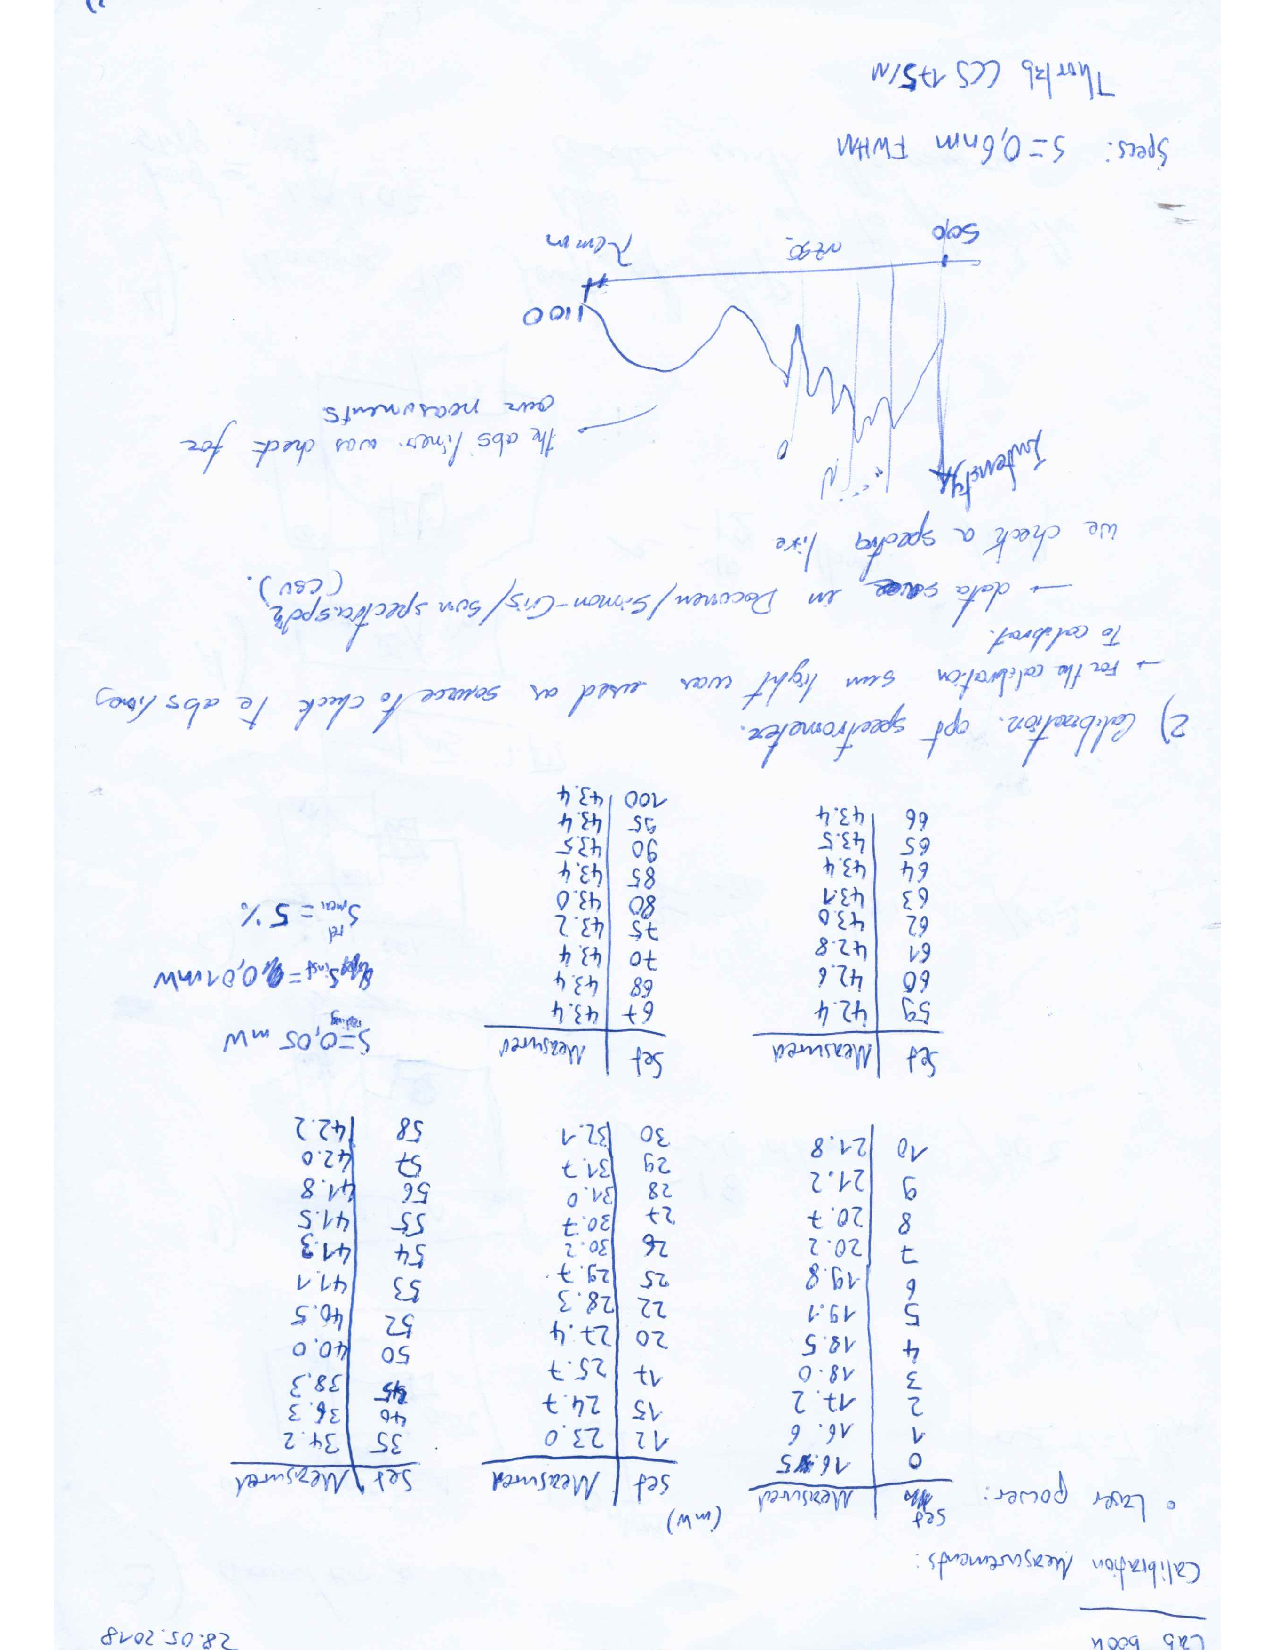
\includegraphics[width=0.9\textwidth,angle=180]{../labbook/labbook-1.pdf}
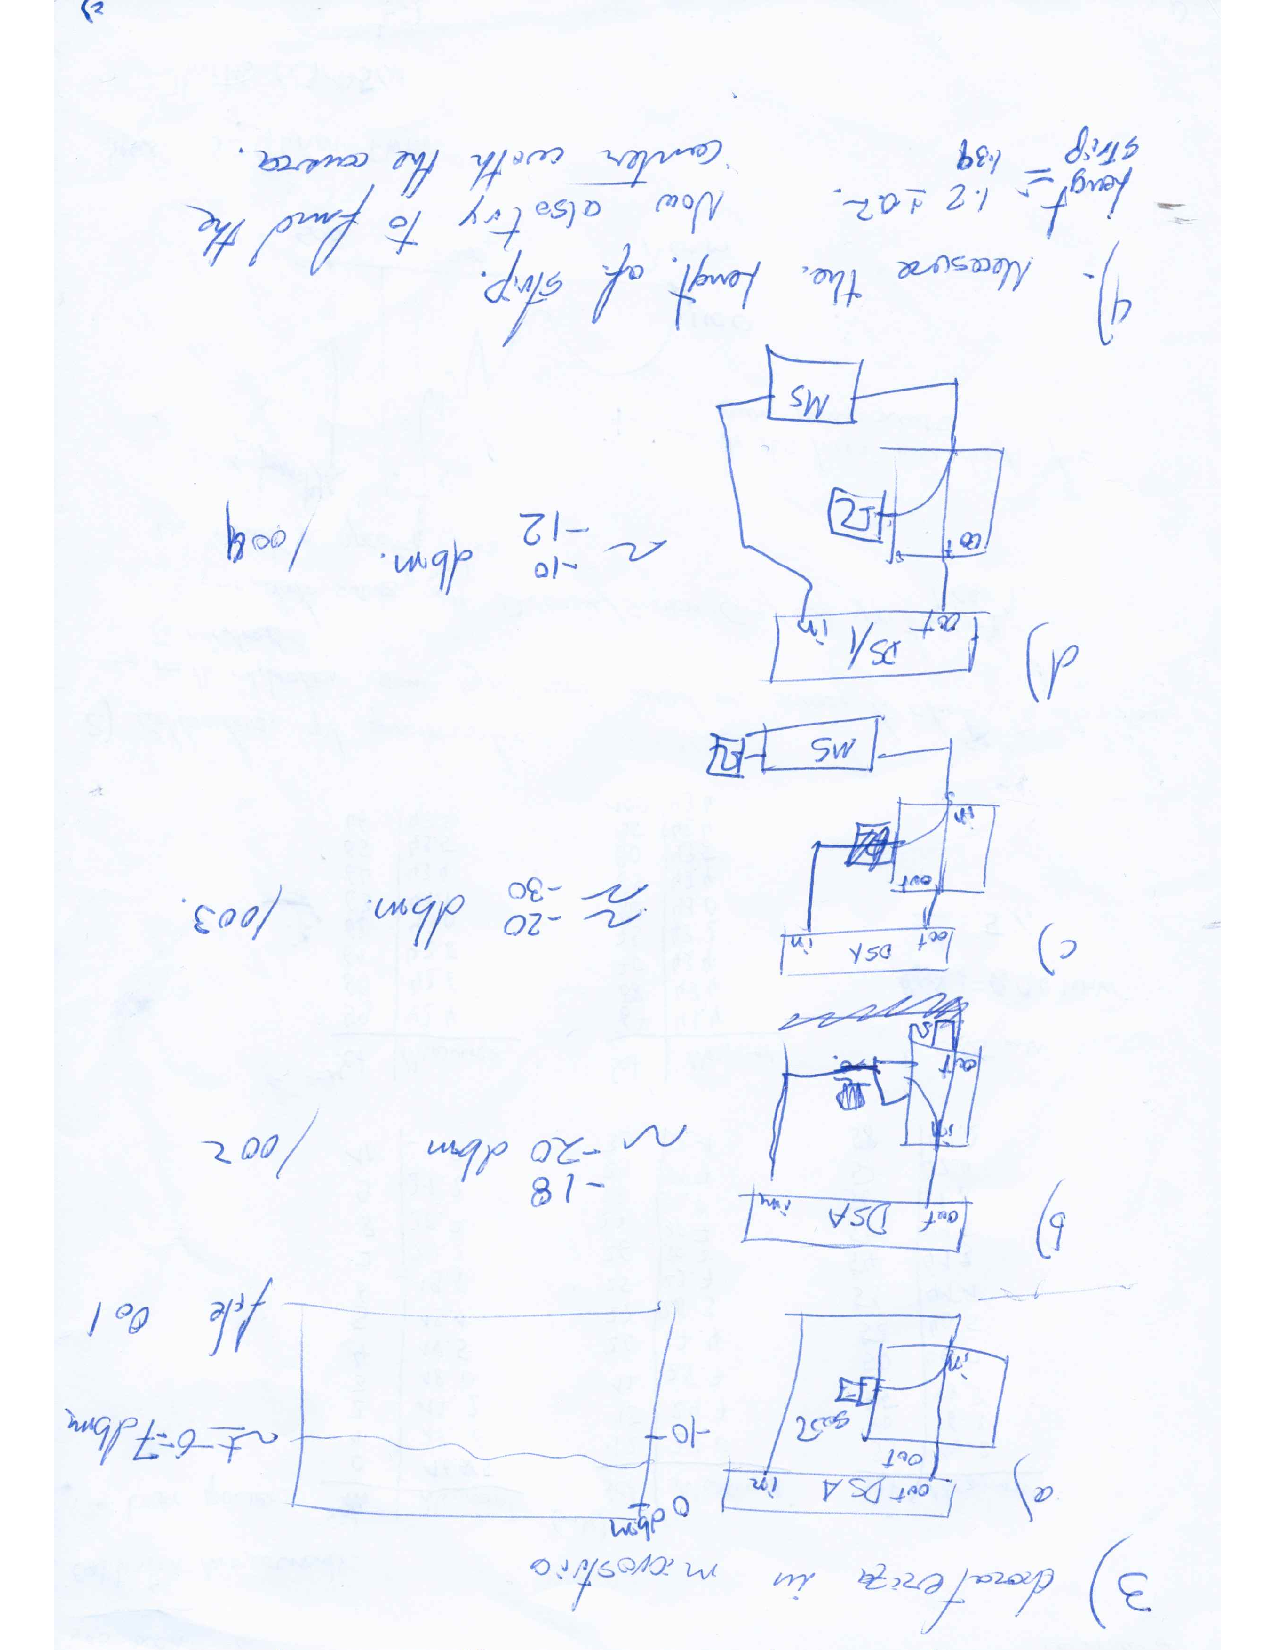
\includegraphics[width=0.9\textwidth,angle=180]{../labbook/labbook-2.pdf}
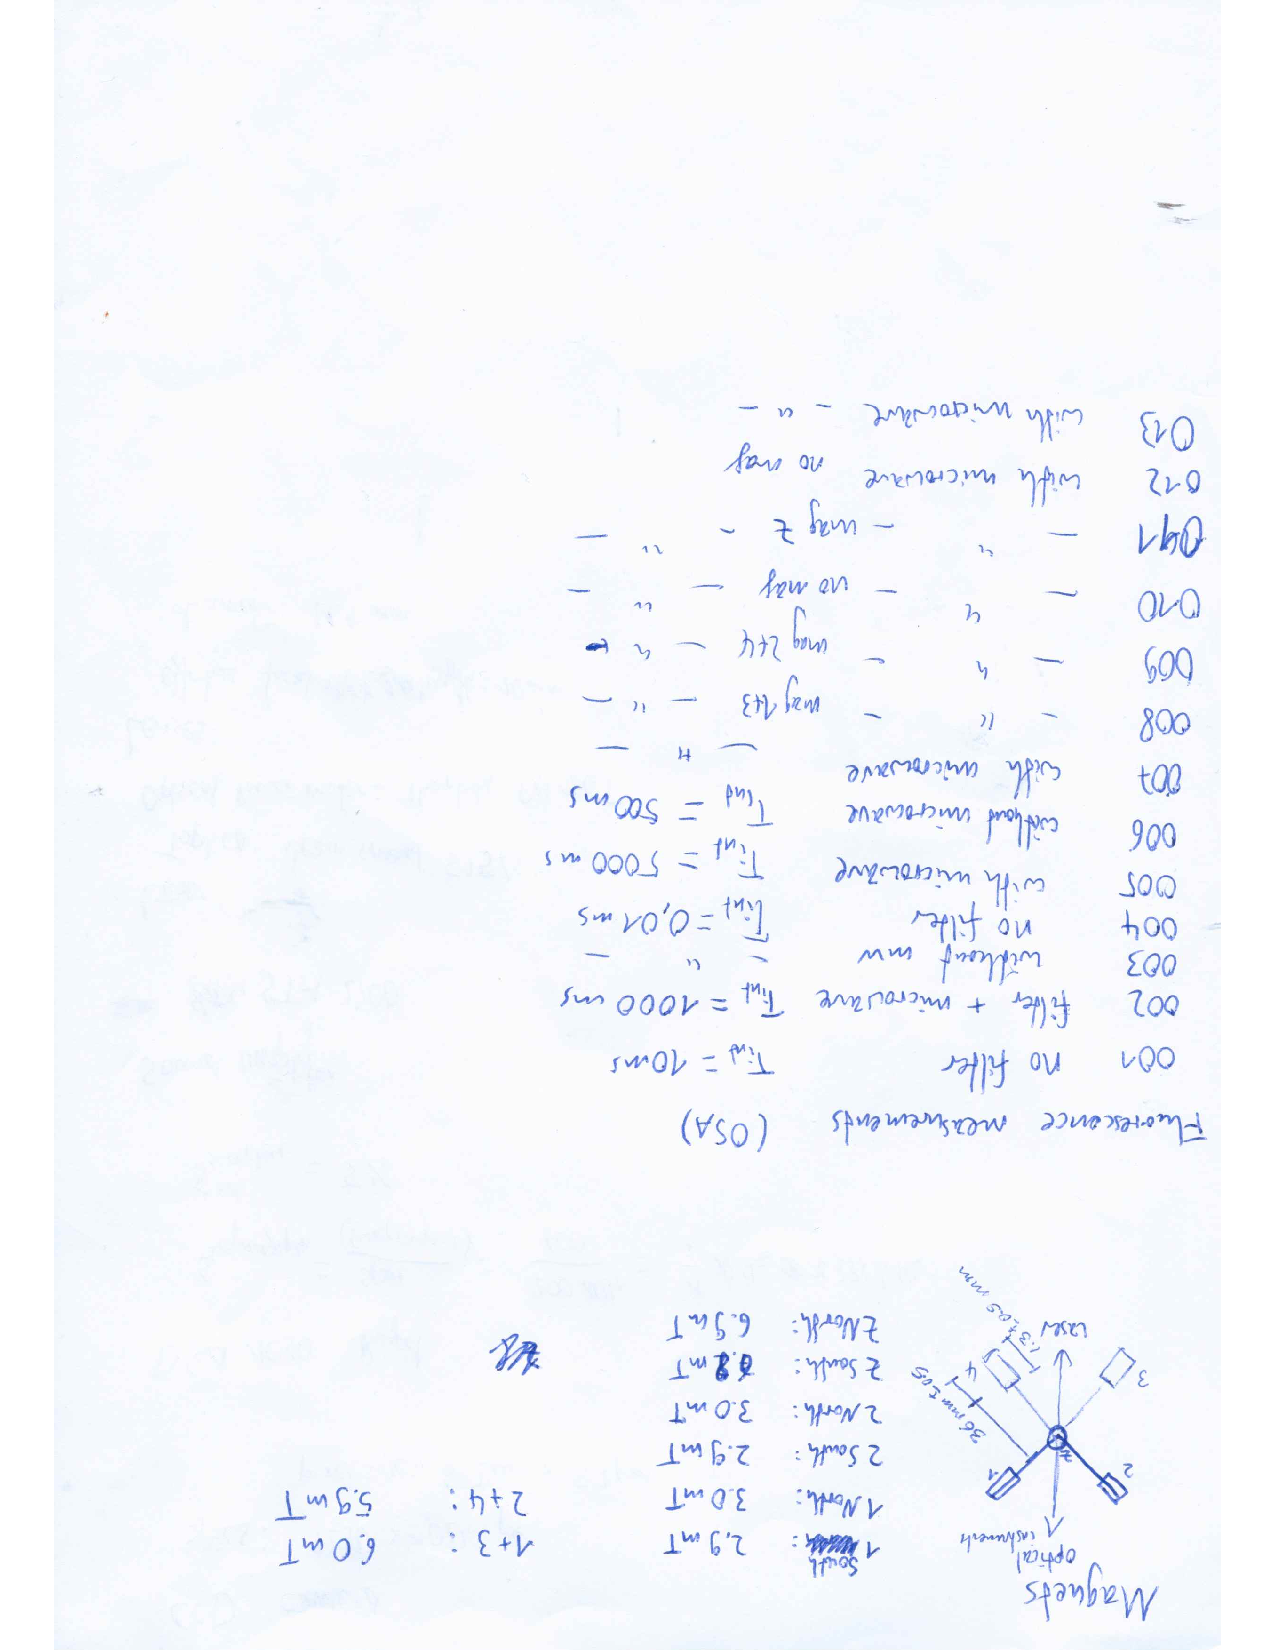
\includegraphics[width=0.9\textwidth,angle=180]{../labbook/labbook-3.pdf}
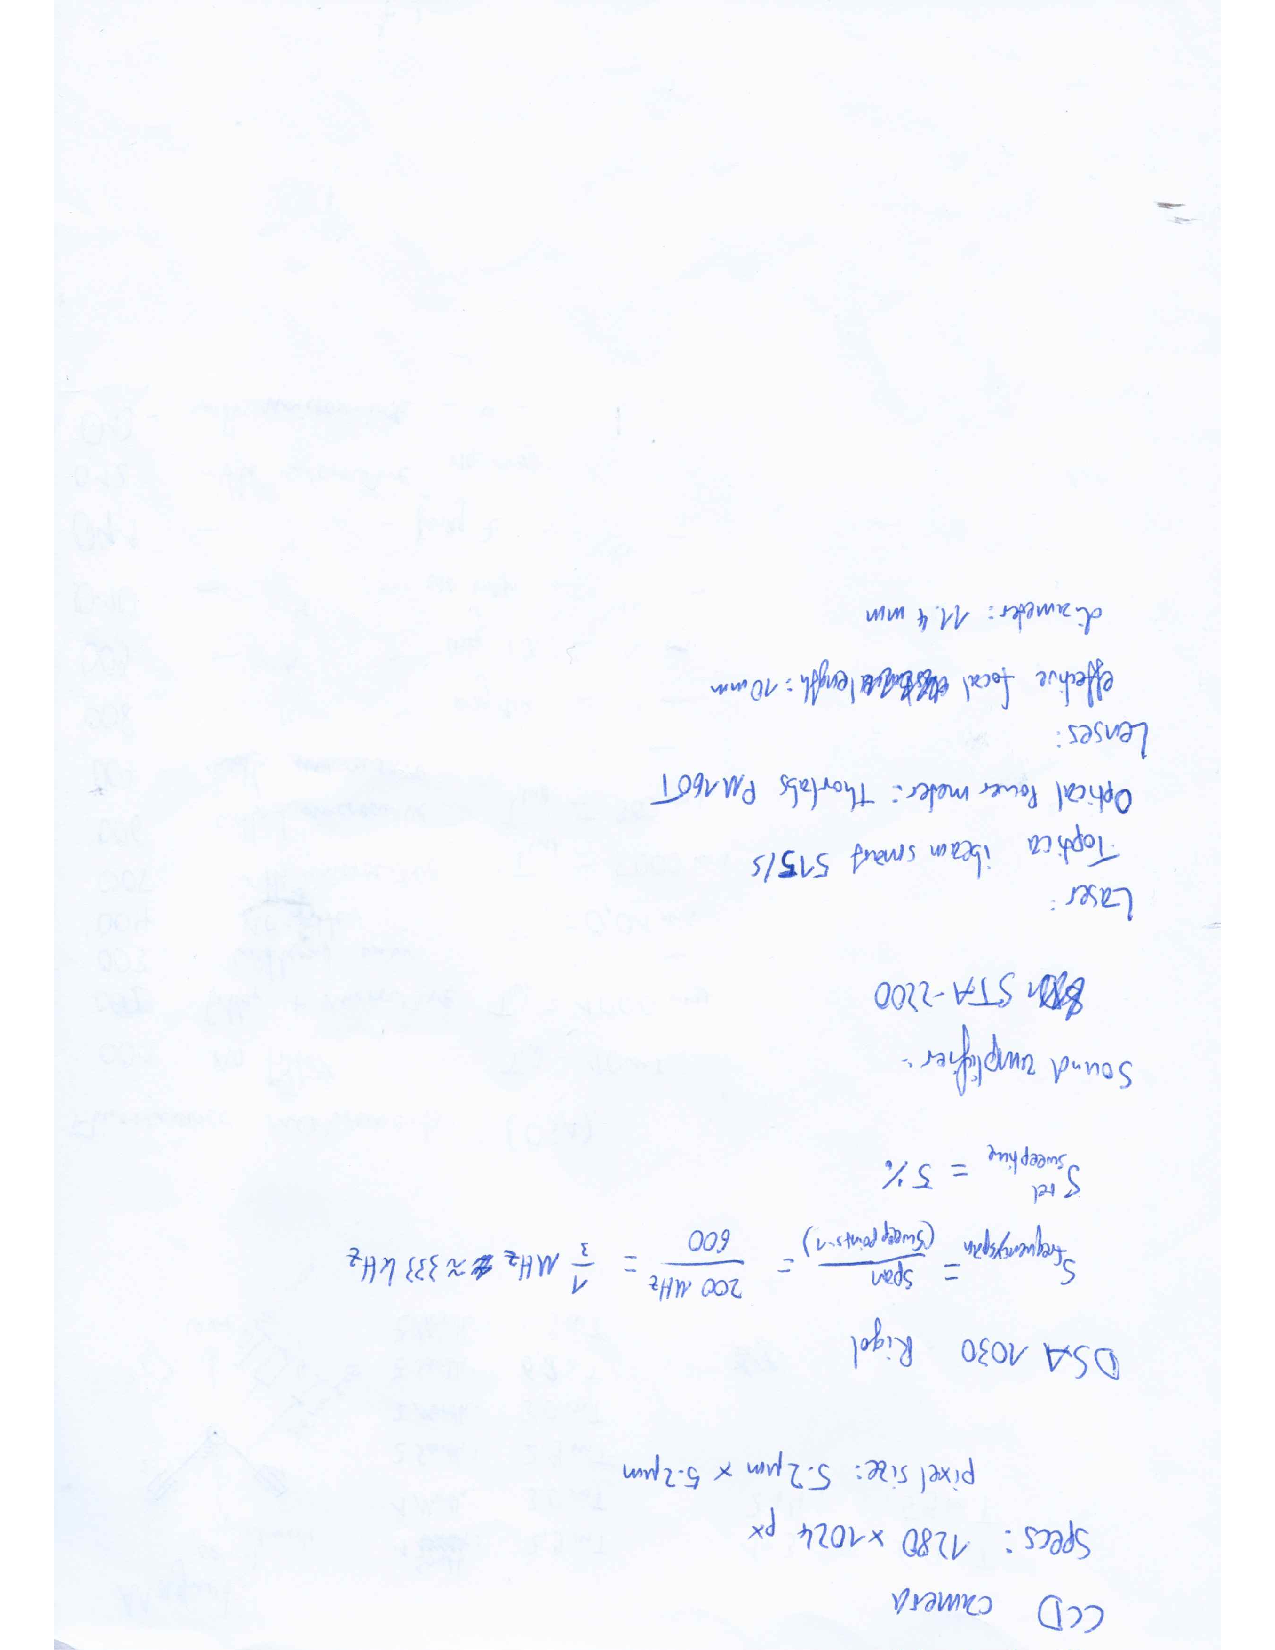
\includegraphics[width=0.9\textwidth,angle=180]{../labbook/labbook-4.pdf}
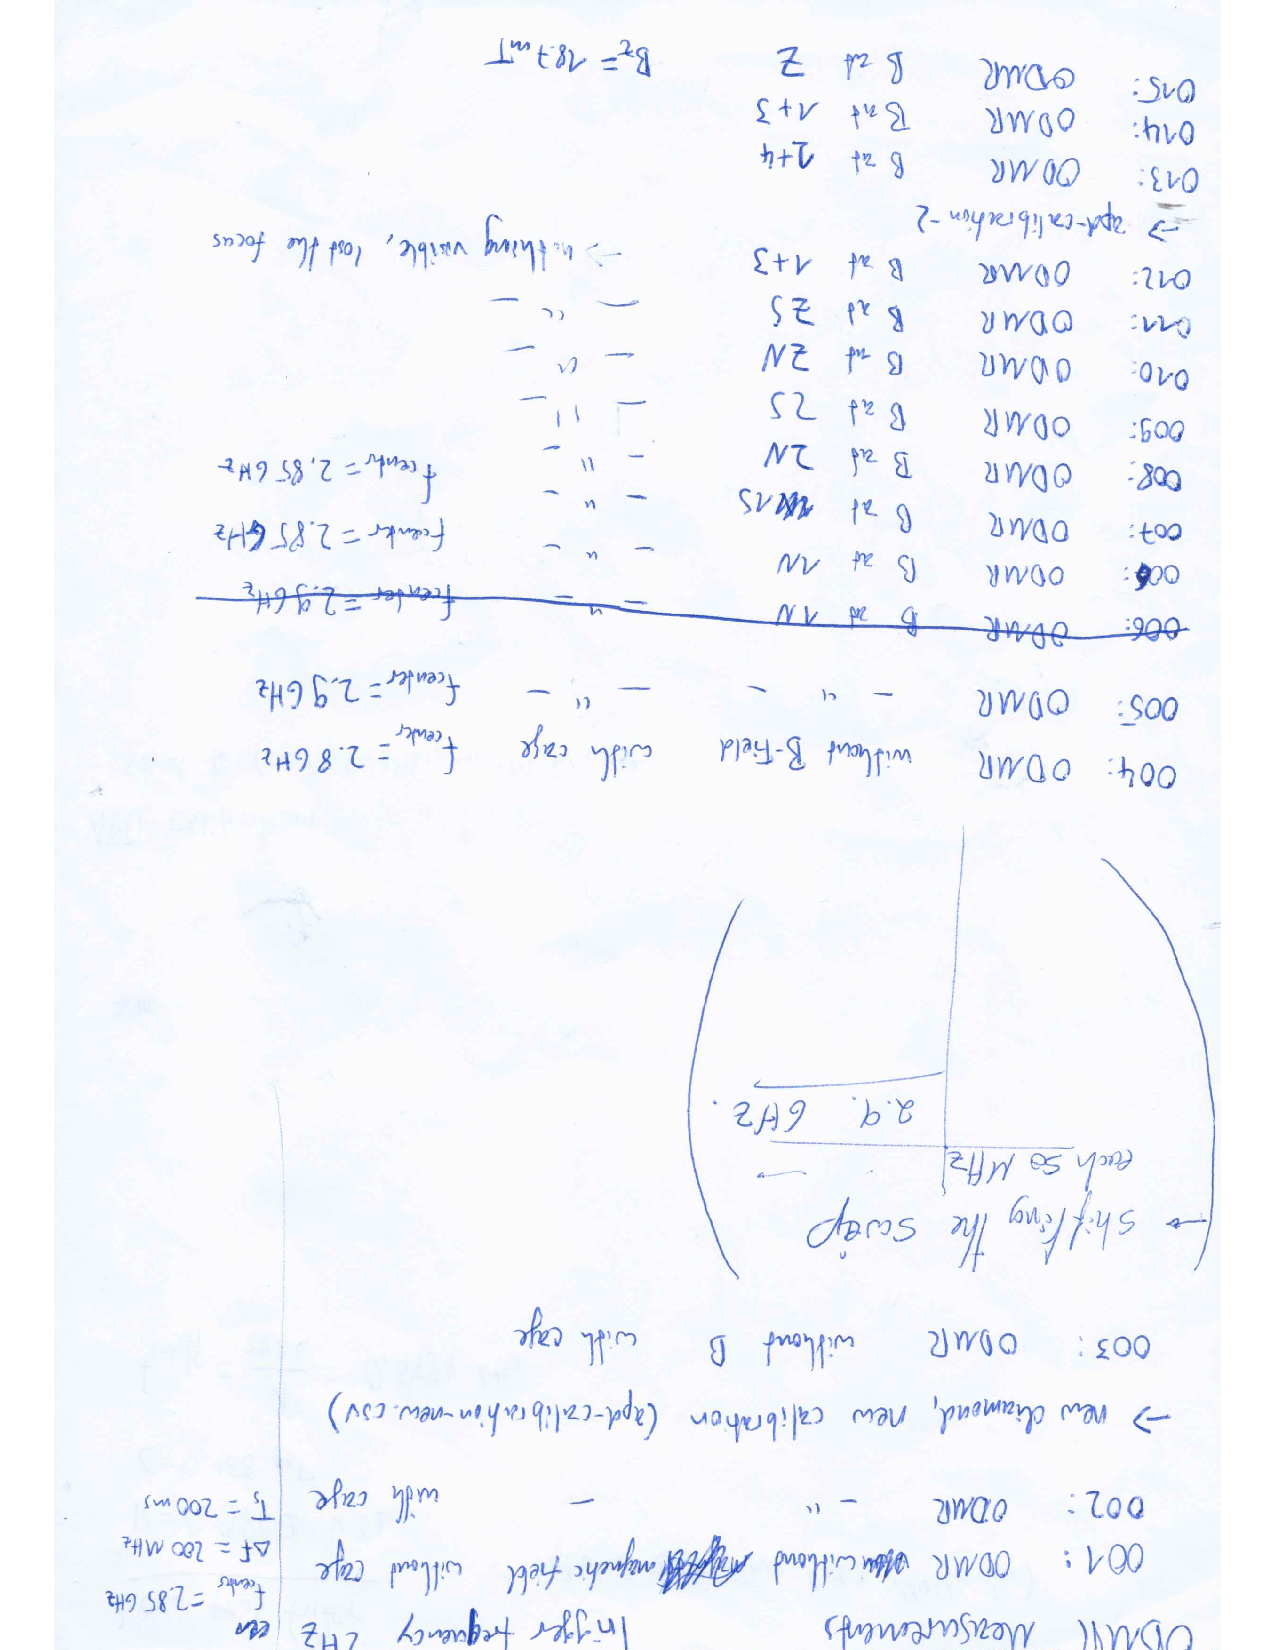
\includegraphics[width=0.9\textwidth,angle=180]{../labbook/labbook-5.pdf}
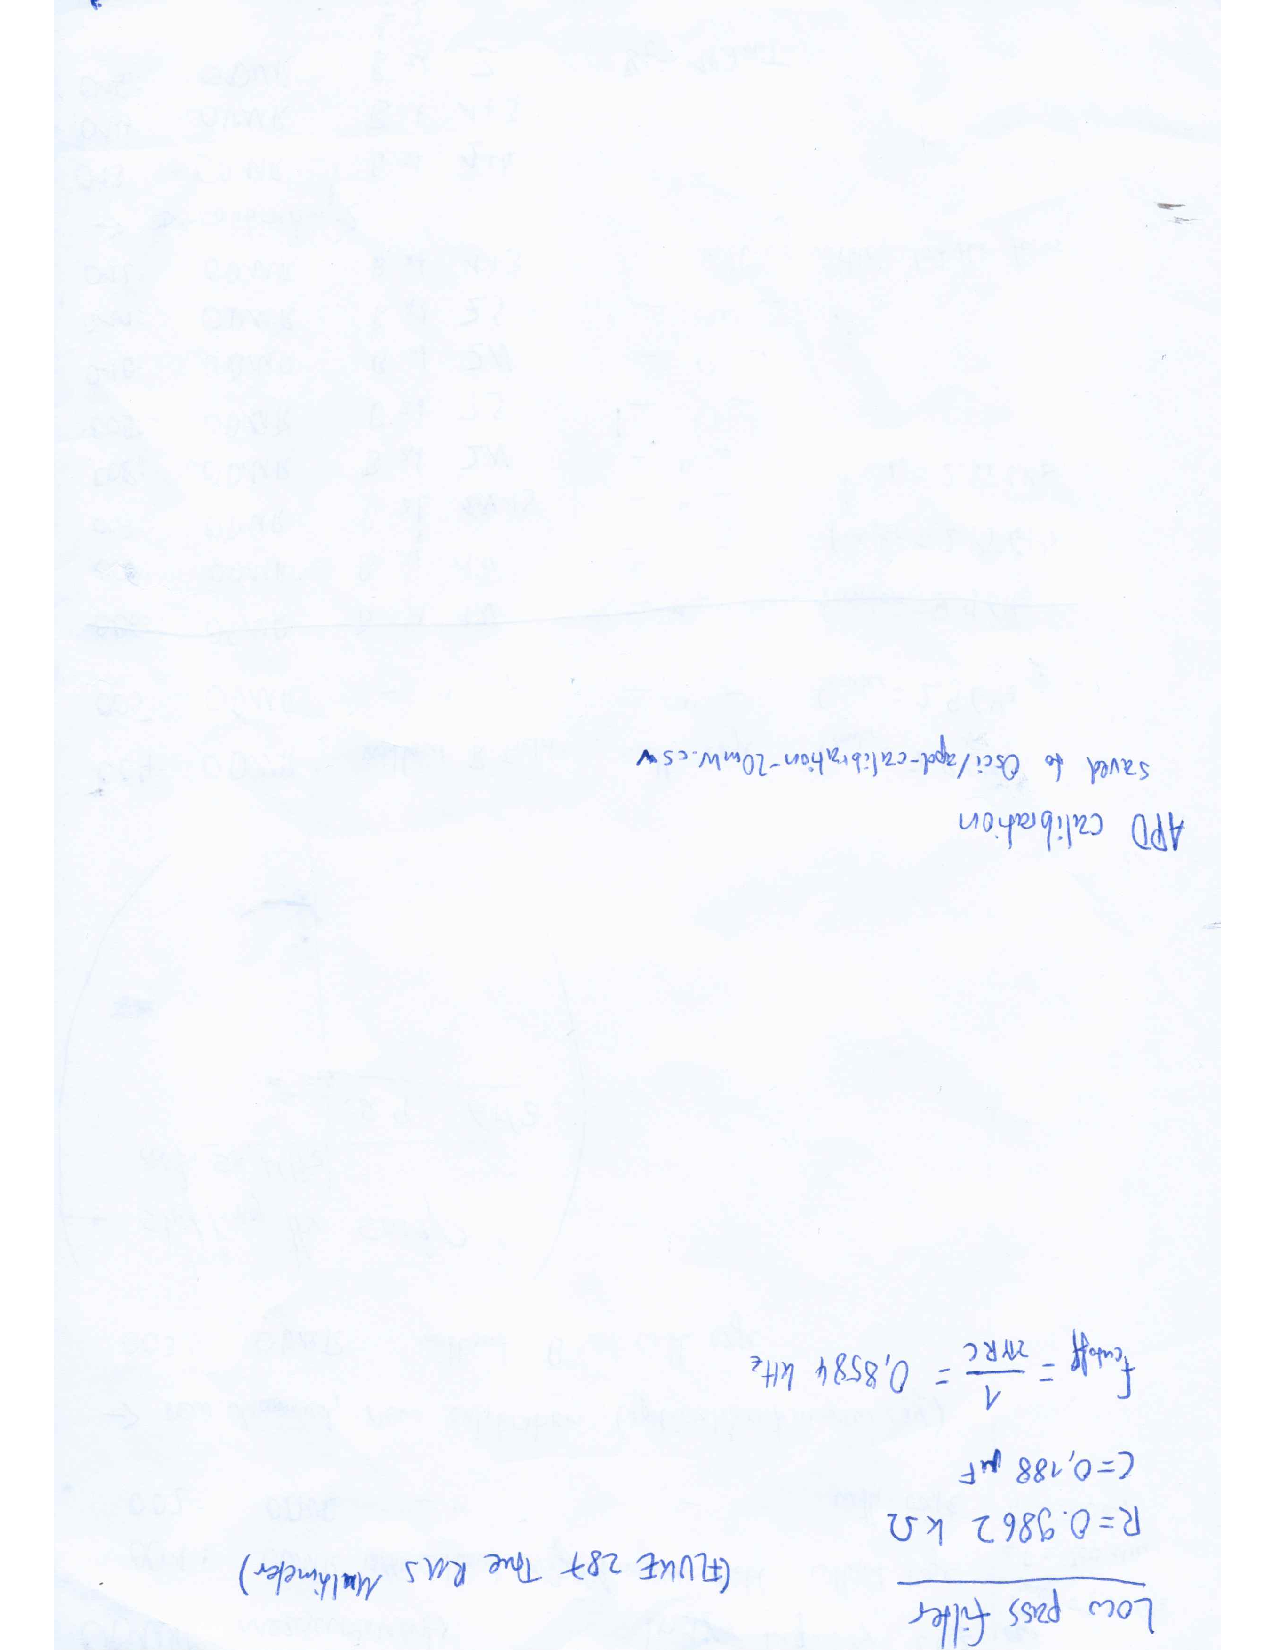
\includegraphics[width=0.9\textwidth,angle=180]{../labbook/labbook-6.pdf}

	\newpage
	\listoffigures
	%\newpage
	\listoftables
	
	%Literatur----------------------------------------------------------------------------------------------------------
	
	%\cite{les}
	\newpage
	\printbibliography[heading=bibintoc]
	

	
\end{document}